\documentclass[a4paper, 12pt]{report}
\usepackage{graphicx} % Required for inserting images
\usepackage[T1]{fontenc}
\usepackage[latin1]{inputenc}
\usepackage{glossaries}
\usepackage{graphicx}
\usepackage{amsfonts}
\usepackage{subfigure}
\usepackage[hidelinks]{hyperref}
\usepackage{pifont}
\usepackage{array}
\usepackage{booktabs}
\usepackage{cleveref}
\usepackage{algorithm}
\usepackage{algpseudocode}
\usepackage{multicol}
\usepackage{eufrak}
\usepackage{amssymb}
\usepackage{listings}
\usepackage{amsthm}
\usepackage{verbatim}
\usepackage{tikz}
\usetikzlibrary{shapes,arrows}
\usepackage{tikz}
\tikzstyle{mybox} = [draw=black, thin, rectangle, rounded corners, inner ysep=5pt, inner xsep=5pt, fill=blue!15]
\newtheorem{theorem}{Teorema}
\usepackage[a4paper, top=2.8cm , bottom=2cm , right=2cm , left=2cm ]{geometry}

\usepackage[table,xcdraw]{xcolor}
\usepackage{array}

\title{
    {\color{black}
    \textbf{  \Huge{MACHINE LEARNING FOR VISION AND MULTIMEDIA} }\\}
    \textit{Lecture notes}
    \linespread{2}
}
\author{Carlo Migliaccio}
\date{AA 2024/2025}

\theoremstyle{definition}
\newtheorem{definition}{Definition}[section]

\pagestyle{headings}

\theoremstyle{remark}
\newtheorem*{remark}{Remark}

\begin{document}
\maketitle
\tableofcontents

\chapter{Introduction}
\chapter{Introduction}
Among the definitions one gives of \textbf{Machine learning} we can say that it is a \textit{"Field of study that gives computers the ability to learn without being explicitly programmed"}. Nowadays, the \textit{Artificial intelligence} is in general that the electricity was in the 19$^\text{th}$ century. Something of paramount importance! \\
There are several methodologies and subfields in Machine Learning and the distinction is based on \textit{how much and how} the human collaborate and of the type of provided data. The most important classification is the one between:
\begin{itemize}
    \itemsep-0.3em
    \item \textit{Supervised learning} (this course), is the approach which uses \textbf{a-priori knowledge} embedded in the data that are used for training algorithms and recognize patterns;
    \item \textit{Unsupervided learning}, is the approach at the opposite whose main feature is not using \textit{labeled data} for assess the tasks.
    \item \textit{Other approaches}. Due to its vastness, in machine learning you can find for sure other subfields. For example the \textit{Reinforcement learning, Semi-Supervised learning, trasnfer learning}. However they are all outside the purposes of this course. 
\end{itemize}

\begin{figure}[h]
    \centering
    
\includegraphics[scale=0.2]{img/AI.jpeg}
\end{figure}

\section{Supervised learning}
From \textsc{Wikipedia (EN)}: \textsf{Supervised learning (SL) is a paradigm in machine learning where input objects (for example, a vector of predictor variables) and a desired output value (also known as a human-labeled supervisory signal) train a model.} In the following we are giving some simple introductory examples about two among the most used techniques in supervised learning.
\subsection{Linear Regression}
Let us imagine we are supposed to create a model that allows us to \textbf{predict the price of an house}. For sake of simplicity and clarity, suppose that our \textit{dataset entries} have one feature (the house size in ft$^2$) and the \textit{price} which represents the \textbf{correct answers}.
Using this data we seek for a model which could predict, given the size of an unknown house, his price (in dollars, \$). Several choices can be made. At first, using either a linear or a nonlinear model and so on. It is remarkable that -- even in such a simple example -- we are facing a \textbf{supervised} problem since the right answers are given! This particular case is a problem of \textbf{regression} since we want to \textbf{predict a continuous valued output}, in our case the price.

\begin{figure}[h]
    \centering
    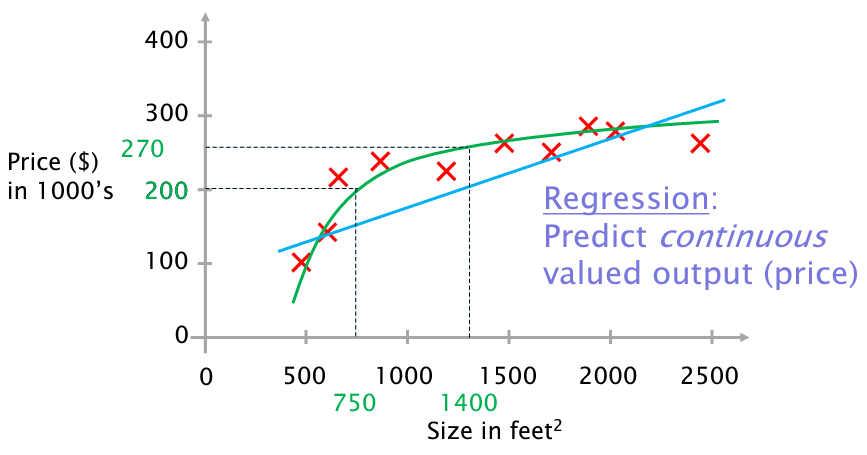
\includegraphics[scale=0.5]{img/prices.png}
\end{figure}

In the figure above is shown the example in which two different models are used, clearly the predicted values for an unknown record is different according to the chosen model.

\subsection{Classification}
On the other hand, when we want to predict a discrete value (eg. YES/NO), we have a \textbf{classification} problem. Again, let us consider a trivial example: we want to predict whether a tumor is malignant or not according to its size. Even in this case we have one feature for the data (\textit{tumor size}) and all the training data are labeled with the YES/NO answer.

\begin{figure}[h]
    \centering
    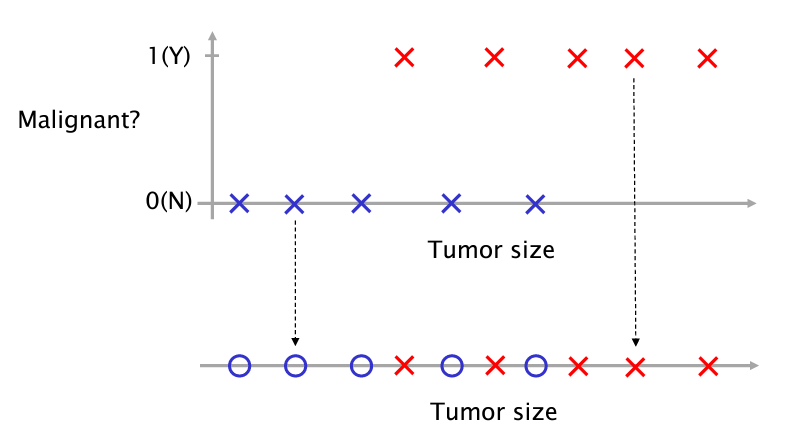
\includegraphics[scale=0.5]{img/tumor.png}
\end{figure}

The figure shows a graphical representation of the dataset. In this case since the answers are associated with different symbols, a more compact representation is given by a one-axis diagram: one feature is given, furthermore a different symbol is associated to different classes. Note that in this case we are in front of a a \textbf{binary classification problem}, in general the classes to predict are not necessarily in number of two. \\
This was just an example to understand and introduce the problem, but in real-world applications, one feature is not sufficient to build a good model! For sake of clarity, let us complicate a little bit the example we have just presented by adding a new feature associated with the \textit{age of the patient}.

\begin{figure}[h]
    \centering
    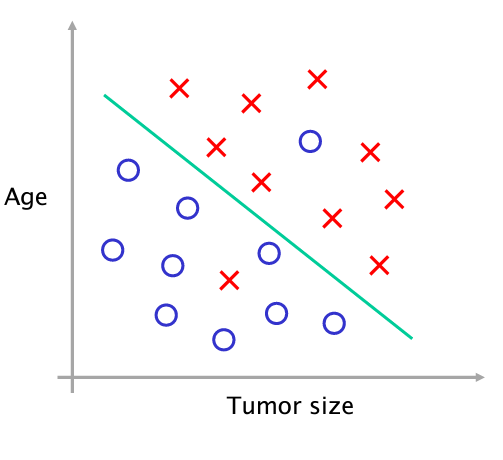
\includegraphics[scale=0.5]{img/tumor_more.png}
    \caption{Bi-variate problem with linear decision boundary}
\end{figure}

In this case the data set is represented in a 2D graph, one axis for each feature and a different symbol for each class. Now, given a record associated with a new patient, what is the class for its tumor? In this case can be useful to individuate a \textbf{decision boundary} according to which one can decide clearly what is the prediction (Positive/Negative). In the two parts there are some outliers, for this reason one can be tempted to build a more "accurate" decision boundary that perfectly split the two classes.

\begin{figure}[h]
    \centering
    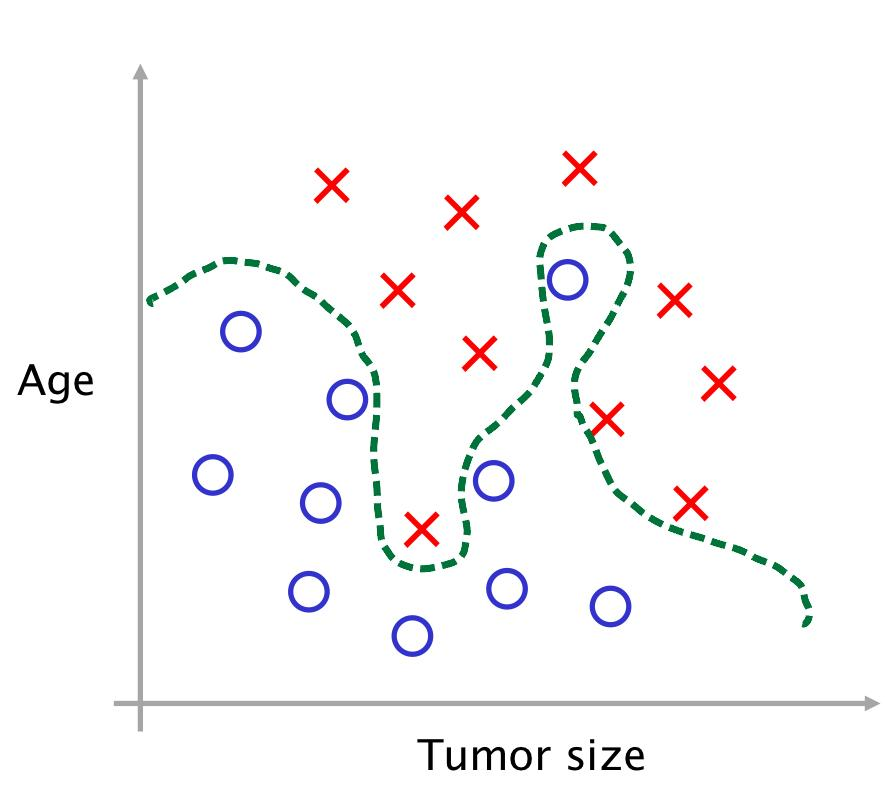
\includegraphics[scale=0.2]{img/overfit.jpeg}
    \caption{Example of overfitting}
\end{figure}

\noindent
Is this a good model for the given problem? NO! This model will have very bad \textit{performances of generalization} with new records to be classified, since it is too much related to the given dataset. In a colloquial way we say that: \textsf{The model has learnt the by heart the dataset}. A problem known as \textbf{overfitting}. \\
Finally, we can say that few features will result in a bad model, on the other hand also too much features will result in a bad model for another problem known as the \textbf{curse of dimensionality}.\footnote{
    In these case techniques of dimensionality reduction has to be employed.
}

\section{Unsupervided learning}
At the opposite of the \textit{supervised approach}, here patterns are learnt exclusively from unlabeled data. The most common example of such an approach is the \textbf{Clustering}.

\subsection{Clustering}
In this case several algorithms are employed to discover groups called \textbf{clusters} associated with objects which are similar in some sense. In general, very often distance-based measures are used to individuate the groups. One of the most famous clustering algorithm is the \textit{K-Mean}. The following figure is an example of bivariate clustered data. 

\begin{figure}[h]
    \centering
    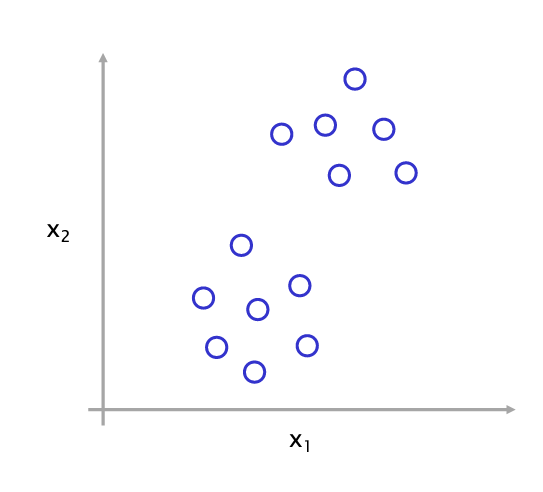
\includegraphics[scale=0.5]{img/clustering.png}
\end{figure}

Unsupervised techniques are used also in bioinformatics in manipulated \textit{DNA microarrays}, for gropuing together similar web pages, for analysis of astronomical data and so on.

\chapter{Model, cost, parameter learning, Gradient Descent }
Let us come back to the first example of \textit{price prediction} and formalize some aspects we have only mentioned. The objective here is to exploit this example to introduce and better clarify several concepts.\\
\section{Model representation}
At first, the training set we are using is something similar to the following:

\begin{table}[h]
    \centering
    \begin{tabular}{c c}
        \textbf{Size in feet$^2$($x$)}&\textbf{Price(\$) in 1000's($y$)}\\
        \hline
        2104&460\\
        1416&232\\
        1534&315\\
        852&178\\
        ...&...
    \end{tabular}
\end{table}
\noindent
We will indicate with $m$ the number of samples of the training set (number of rows), $x$ is the input (possibly multivariate) variable, $y$ is the output variable, $(x,y)$ indicates generically a sample from the training set, while $(x^{(i)}, y^{(i)})$ indicates the $i$-th sample of the training set.

\begin{figure}[h]
    \centering
    \label{}
    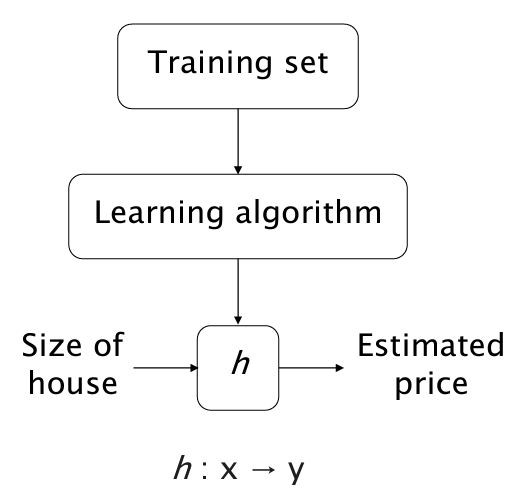
\includegraphics[scale=0.5]{img/model.png}
    \caption{Scheme for model construction (price prediction)}
\end{figure}

The figure above shows schematically the steps in order to produce a certain model for the analysed case-study. Very briefly, a \textbf{training set} is used by a \textbf{learning algorithm} to obtain an \textit{hypotesis} $h_\theta(x)$ which is later used for the prediction.\\
In the case we want to solve a \textbf{univariate linear regression problem} the hypotesis $h$ has got the shape:
\begin{equation}
    h_{\theta}(x)=\theta_0+\theta_1{x}
\end{equation}
where $\theta_0$ and $\theta_1$ are the parameters of the line.\footnote{
    We can imagine them as two handles to: move up/down the line ($\theta_0$) and to rotate it ($\theta_1$).
} We call \textit{univariate} the the problem since we have only one feature and it is a \textit{linear regression} because we want to predict the price (output) according to a line.\footnote{
    Note that in case of a \textbf{neural network} the parameters and the hypotesis assume a different notation. In particular the hypotesis becomes the \textit{predicted value} indicated with $\hat{y}$, the parameters are split in a \textbf{bias}, indicated with $b$ whose role is the one played by $\theta_0$, while the $\theta_i$, $i=1,...,n$ are the weights $w_i$
 }
\textbf{Question: How can we choose $\theta_0, \theta_1$?} Intuitively one can choose the parameters associated with the line $h_\theta(x)$ which is as closest as possible to the given $y$. Very often these parameters are the ones which solve the following problem: 
\begin{equation}\label{eq:ls1}
    \min_{\theta_0, \theta_1} {\frac{1}{m} \sum_{i=1}^{m}{
        \frac{1}{2} \bigl(
            \underbrace{h_\theta(x^{(i)})}_{\textsf{predicted value}}-
            \underbrace{y^{(i)}}_{\textsf{actual value}}
            \bigr)^2
    }}
\end{equation}
The function $\frac{1}{2} (
    h_\theta(x^{(i)})-y^{(i)})^2$ is the \textsf{Loss}($h_\theta(x), y$) or \textsf{Cost}($h_\theta(x),y$).  If we call $J(\theta_0, \theta_1)$ the argument of the minimization problem the (\ref{eq:ls1}), the problem to solve can be expressed as
\begin{equation}\label{ls2}
    \min_{\theta_0, \theta_1} {J({\theta_0, \theta_1})}
\end{equation}
Summarizing: we want to perform a prediction using the hypotesis $h$ which is dependent on parameters $\theta_0, \theta_1$ which are issued by minimizing a certain functional $J(\theta_0, \theta_1)$. Let us investigate better on the role of $J$ in this supervised learning task.\\
At first -- for sake of simplicity -- we can eliminate a degree of freedom fixing the parameter $\theta_0$ to be (without loss of generality) $\theta_0=0$. For each choice of $\theta_1$ we will obtain a $h_{\theta_1}(x)$. If we compute $J(\theta_1)$ (for each $\theta$) will obtain a certain univariate function $J(\theta_1)$, the minimization of which will give us the \textit{optimal} $\theta_1$ parameter for our hypotesis. An example is shown in the following figure:

\begin{figure}[h]
    \centering
    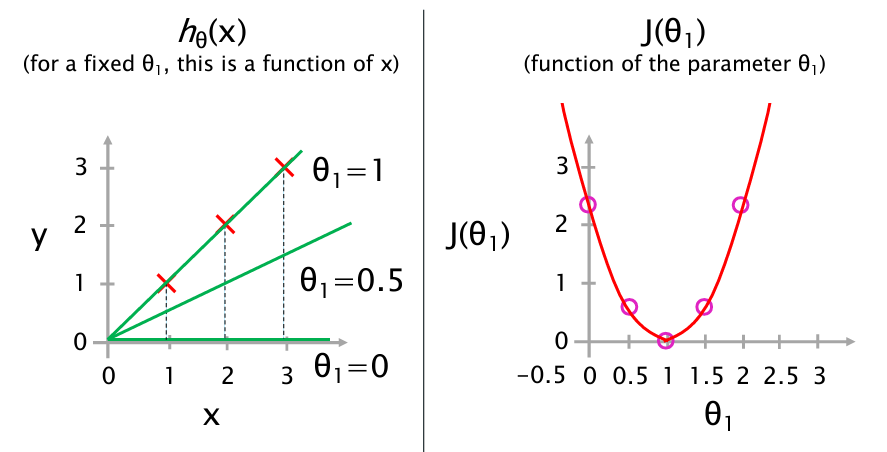
\includegraphics[scale=0.7]{img/J_univariate.png}
\end{figure}
\noindent
Analyzing the complete model, we have two degrees of freedom (DOF) since  $\theta_0, \theta_1$ can vary. In this case the functional to be minimized has to be represented in a 3D space, then we obtain a surface similar to one presented in the following figure:

\begin{figure}[h]\label{fig:surface}
   \centering
   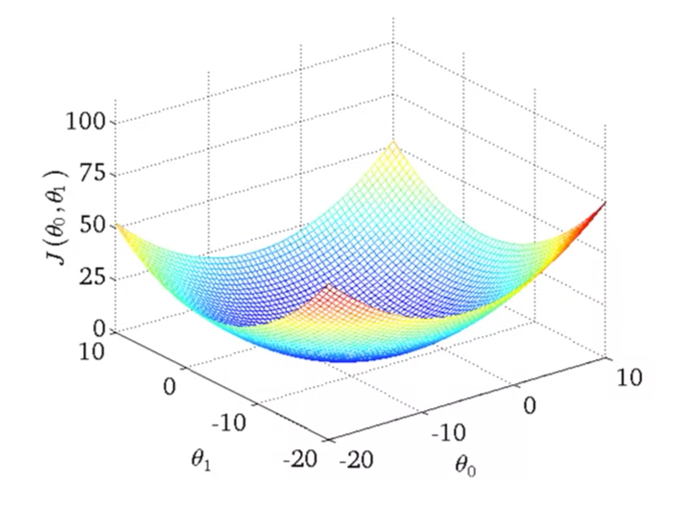
\includegraphics[scale=0.7]{img/J_bivariate.png} 
   \caption{Example of $J(\theta_0, \theta_1)$}
\end{figure}

In the common case of bivariate minimization problem one can use \textit{contour plot} which analyze the shape of the function at different heights. It is remarkable that points in the space $(\theta_0, \theta_1)$ which are on the same \textit{countour line} result in very different hypotesis. It is trivial to understand that,  in this case the minimum $J(\theta_0, \theta_1)$ is attained on the bottom of such a \textit{bowl-shaped} surface.

\begin{figure}[h]
    \centering
    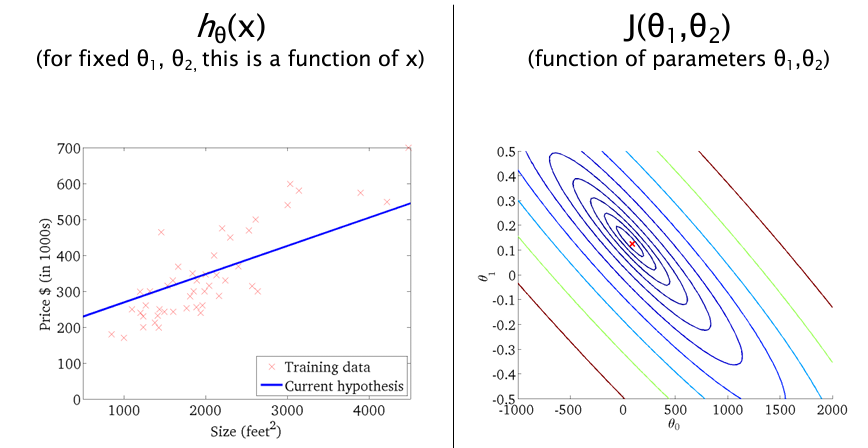
\includegraphics[scale=0.7]{img/contour.png}
\end{figure}

\section{Parameter learning: Gradient descent}
The objective here is to find a way to minimize a certain multivariate functional $J(\theta_1,..., \theta_n)$, the idea is using some methods that iteratively bring us to the minimum according to a certain criteria. In this paragraph we analyse the \textbf{Gradient Descent} algorithm, the main idea here is to start with some $\theta_0, \theta_1$\footnote{
    They are chosen either randomly or $\theta_i=0, \ \forall i$.
}, and keep changing them until $J$ evaluated at those parameters could reach (hopefully) the minimum, in the gradient descent this change is made up on the basis of the direction dictated by the \textbf{gradient of the functional} computed at the current parameters value (from which the name). The algorithm for GD is simply as follows:

\begin{figure}[h]
    \centering
    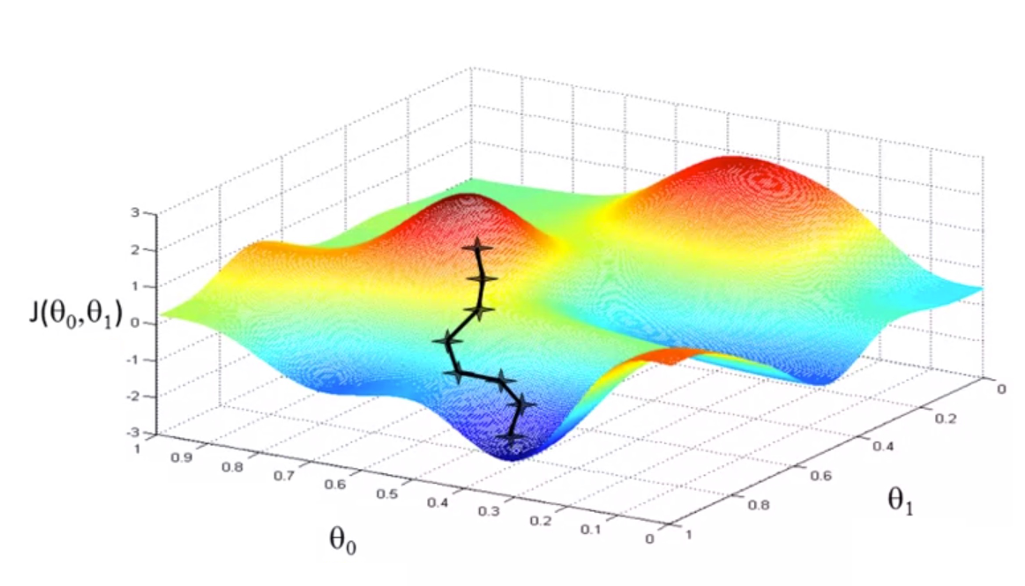
\includegraphics[scale=0.5]{img/nocvx_surf.png} 
\end{figure}

\begin{algorithm}[h]
    \caption{Gradient Descent}
    \begin{algorithmic}
        \While{!convergence}\\
           $\theta_j:=\theta_j-\alpha{\frac{\partial}{\partial{\theta_j}} J(\theta_0, \theta_1)}$
           \Comment{for $j$=0, $j$=1,...}
        \EndWhile
    \end{algorithmic}
\end{algorithm}

\noindent
The $:=$ symbol is associated with a \textit{simultaneous update}, note that if you put together for each $j$ the partial derivatives of $J$ you will obtain the gradient. The parameter $\alpha$ is called the \textbf{learning rate} and it must be properly chosen because:
\begin{itemize}
    \itemsep-0.2em
    \item If $\alpha$ is \textbf{too small}, then the convergence to the minimum (within a certain tolerance) could be very slow;
    \item If $\alpha$ is \textbf{too large} the algorithm can overshoot the minimum either failing to converge, or diverging.
\end{itemize}
Even when the learning rate is fixed the GD can converge to a (local) minimum since we are moving toward \textit{steep} directions which decrease the functional over time. If we apply the algorithm to the functional of the problem in (\ref{eq:ls1}) we obtain:
\begin{equation}
    \begin{aligned}
        &\theta_0=\theta_0-\alpha{\sum_{i=1}^{m}{(h_\theta(x^{(i)}-y^{(i)}))}}\\
        &\theta_1=\theta_1-\alpha{\sum_{i=1}^{m}{(h_\theta(x^{(i)}-y^{(i)}))} x^{(i)}}
    \end{aligned}
\end{equation}
this is known as \textbf{batch gradient descent} since for each step we use all the training samples. There are cases in which the minimization is particularly 'simple'. This happens when the functional is convex in $\theta$. Besides, for the class of convex functions a local minima is also a \textbf{global and only min}.

\section{Multivariate linear regression}
It is quite immediate to understand that the linear regression can be used also for a \textit{multivariate context} in which the samples are characterized by many features. In this context the hypotesis becomes:
\begin{equation}\label{eq:multivariate}
    h_\theta(x) = \theta_0{x_0}+\theta_1{x_1}+...+\theta_n{x_n}=\theta^T{x}
\end{equation}
In this case we have $n$ parameters and associated features $x_i$, so that the functional $J$ is function of $n$ parameters, in this case the partial derivatives to compute, obviously, will increase. Note that a \textit{fictitious} feature $x_0=1$ has been added with the purpose to employ a vector notation.\footnote{
    The great majority of tools and softwares which are used for machine learning exploit vector and matrices calculus to carry out their work.
}\\

\section{Data mean normalization}
Sometimes, before starting with the model construction, some preliminary operations are needed. For example, often it is better for the features being on a \textbf{similar scale}. In this  case we replace in each sample for each feature $x_i=x_i/s_i$ where $s_i$ can be either the range (max-min) for that feature or some index similar to variance/standard deviation.\\
Other times, one is supposed to normalize the data so that they can have a \textit{zero mean}. The trick here is replacing $x_i=x_i-\mu_i$, where $\mu_i$ is the mean for the $i$-th feature. Not rarely, you can find the two transformation combined such thet
\begin{equation}
    x_i=\frac{x_i-\mu_i}{s_i}
\end{equation}

\section{Debug of Gradient Descent algorithm}
The \textit{gradient algorithm} is clearly a descent method in the sense that -- being $k$ the $k$-th iteration -- it holds that $J(\theta_{k+1}) < J(\theta_{k})$, this is the same to state that the $J(\theta)$ function is required to be strictly decreasing. An \textbf{automatic convergence test} can be performed: for example the objective function $J$, had had a decreasing less than a certain threshold $\varepsilon=10^{-3}$ (for example).\\
Whether the algorithm is not working well the value for the \textbf{hyperparameter} $\alpha$ must be changed (for example decreasing it). One way to choose \textit{manually} $\alpha$ is by \textit{trial-error}\footnote{
    A more accurate method is the \textbf{backtracking line-search} which repeat some calculations until the so-called \textit{Armijo condition} is not met; however it requires that additive hypotesis are made on the regularity of the objective and its gradient.
}, choosing the $\alpha$ in a range and then plotting $J(\theta)$ as a function of the number of iterations. 

\begin{figure}[h]
    \centering
    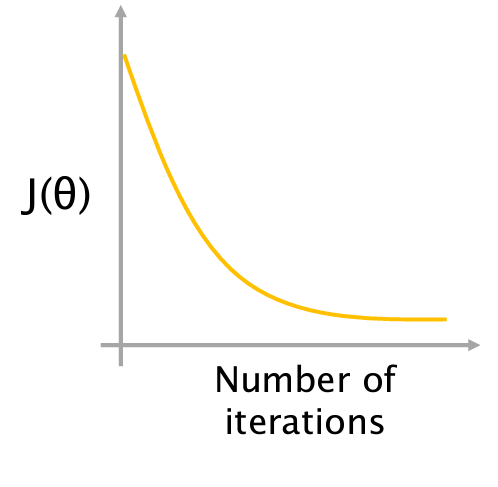
\includegraphics[scale=0.6]{img/alpha.png}
    \caption{Desired behaviour for $J(\theta)$ vs \# iterations}
\end{figure}
 
\section{Alternative to Gradient Descent}
There are alternative methods to gradient descent, for example the normal equation method which is derived by the analytical solution of the well-known \textbf{least-squares} problem. In this case $\theta$ is found by solving the system (normal equations):
\begin{equation}
    (X^T X)\theta = X^T{y}
\end{equation}
where the $X$ matrix contains the dataset features and $y$ is the vector with the "right answers". The solution of such a problem gives \textit{one-shot} the solution without proceeding by step as in the case  of gradient descent. The main limitation of such a method is the inversion of the matrix $X^T X$, which could be significantly slow if $n$ (number of features and parameters) is very large.\footnote{
    It is sufficient to think about the number of parameters involved in a problem of image classification. They are in a number of 3 billion for an RGB $1000\times1000$ image. 
}

\section{Polynomial regression}

\chapter{Logistic Regression}

The objective here is discussing the \textbf{Logistic regression} model which is used for \textbf{binary}, and also, \textbf{multiclass classification}. We will start from the hypotesis $h_\theta(x)$ used in the case of regression, we will analyze the aspects which will be maintained of it, and also the cons. 

\section{Classification vs Regression}
Coming back for a while to the problem of \textit{tumor classification}, suppose that a linear hypotesis can be used in order to separate the data. The comprehension of this concept is aided by the following figure: 
\begin{figure}[h]
    \centering
    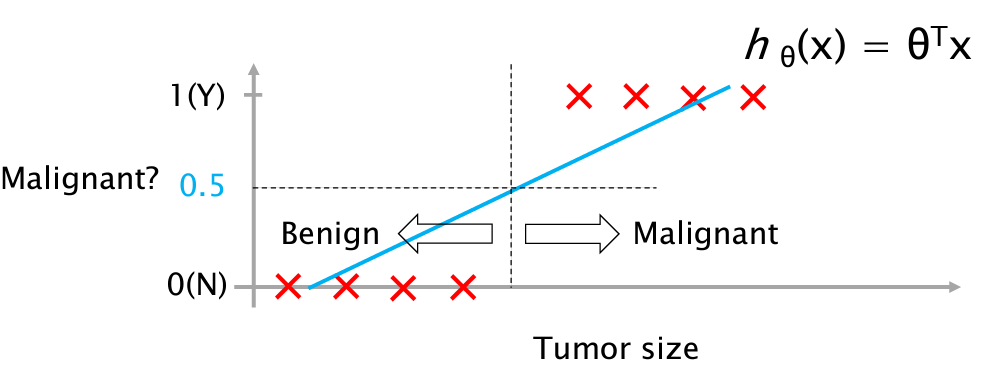
\includegraphics[scale=0.5]{img/Class_vs_Reg.png}
    \caption{Classification with linear hypotesis}
\end{figure}
The hypotesis $h_\theta(x)$ used in order to separate the two class is the line showed in blue. Since here we are not in the case of prediction of a continuous value, we have to find a way for shrink all possible output from the hypotesis in two values (Positive/Negative). At this point an idea could be using a threshold according which you can separate data from the two classes, that is:
\begin{equation} \label{eq:criteria}
    y=\begin{cases}
        1&\text{if} \ h_\theta(x)>0.5\\
        0&\text{if} \ h_\theta(x)\le{0.5}
    \end{cases}
\end{equation}
This appproach seems to work, until we do not change the data used for building the model. Let us consider, for example, the following scenario:
\begin{figure}[h]
    \centering
    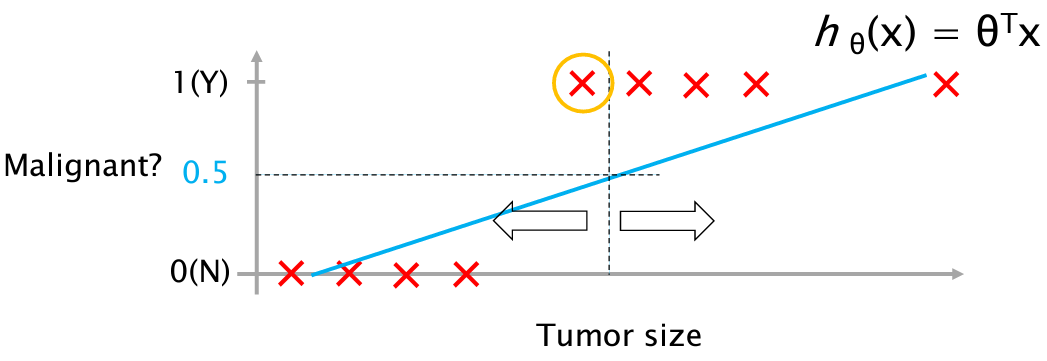
\includegraphics[scale=0.5]{img/Class_vs_Reg2.png}
    \caption{Effect of changing the dataset}
\end{figure}
It appears quite evident that one of the data for which we know that belongs to the positive class, is classified as negative.\\
This is not the only problem: we want that the predicted output\footnote{
    Later we will call it $\hat{y}$, for comparing it to the true output $y$.
}, that is the hypotesis is between 0 and 1, despite the fact of using a threshold this is not satisfied, since a linear function is \textit{unbounded}. At this point our reasoning leads to the formulation of the following two issues:
\begin{enumerate}
    \item A \textit{linear hypotesis} is not suitable for a classification problem, the performances would be awful also on the training set; 
    \item It is required that $$ 0 \le h_\theta(x) \le 1$$ this is not happening in the cases a linear hypotesis is employed.
\end{enumerate}
These are the main points that leads to the \textit{correct formulation} of \textbf{logistic regression}\footnote{
    The name \textit{logistic} is related to the fact that we are solving a dicotomic/binary classification problem.
}.

\section{Logistic regression}
The main concept behind \textit{logistic regression} is using a nonlinear function that saturates the hypotesis between 0 and 1. Basically we have to apply such a function which we will call $g(z)$ to the linear $\theta^T{x}$, such a function is called \textbf{sigmoid} or \textbf{logistic function}. It is depicted in the following and its expression is:
\begin{equation}
    g(z)=\frac{1}{1+e^{-z}}
\end{equation}

\begin{figure}[h]
    \centering
    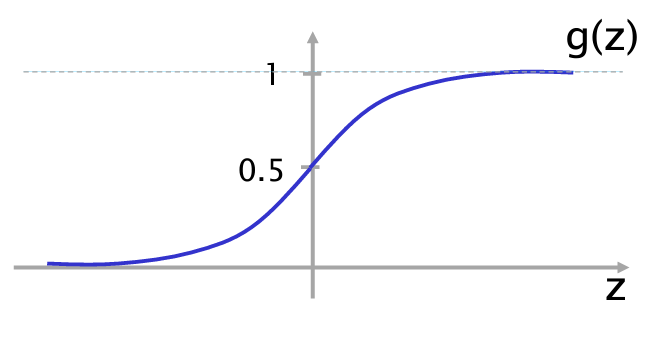
\includegraphics[scale=0.7]{img/logit.png}
    \caption{The logistic function $g(z)$}
\end{figure}

The output of such an hypotesis can be interpreted as \textit{the probability that the output y=1 on a given input x}, for example in the case of tumor classification a value of 0.7 of the hypotesis results in a prediction that for 70\% the given tumor (with its feature is malignant). In order to be mathematically formal we can say that 
\begin{equation}
    h_\theta(x)=P(y=1 | x; \ \theta )
\end{equation}
which is read "the probability for the output $y$ to be 1, given $x$, parametrized by $\theta$. Clearly, at the opposite we can compute
\begin{equation}
    P(y=0 | x; \ \theta) = 1 -P(y=1 | x; \ \theta )
\end{equation}
Here we can stick to the fact of having a threshold. More specifically, we use as an hypotesis $g(\theta^T{x})$ and we can use the criterion used in (\ref{eq:criteria}). Moreover for the particular function  $g(z)$ it is used we can say that, given the features $x$ then it is classified as positive if $\theta^T{x}\ge0$ or negative if $\theta^T{x}<0$, since the counterimage of 0.5 through $g(z)$ is equal to 0, as showed in the following figure.

\begin{figure}[h]
    \centering
    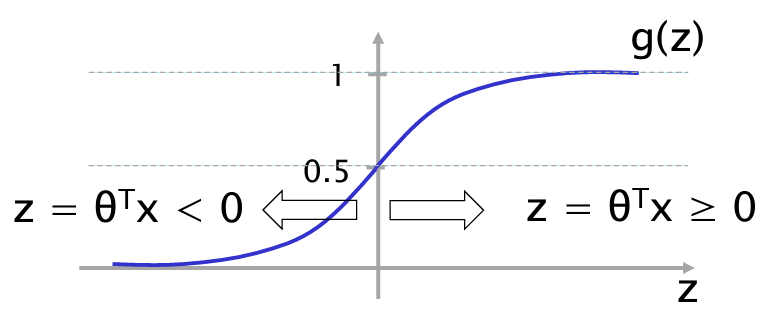
\includegraphics[scale=0.7]{img/logit2.png}
\end{figure}

It appears clear that the linear combination $\theta^T{x}$ is a (linear) \textbf{decision boundary} since it provides us with the information of having a positive or negative record. It is useful to give an example of this fact: 

\begin{figure}[h]
    \centering
    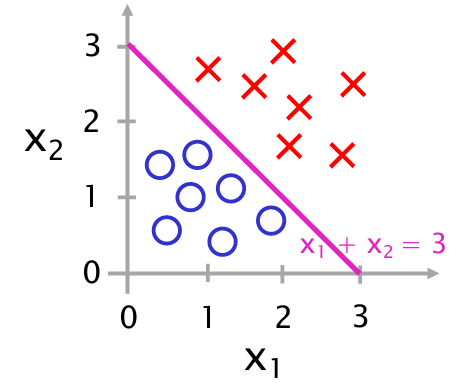
\includegraphics[scale=0.7]{img/decision_boundary1.png}
    \caption{Decision boundary}
\end{figure}

\noindent
Suppose we trained the model and the parameter theta resulted in being $\theta=[-3\  1 \ 1]^T$, this is the same to say that we assign \textit{positive class}to records with feature $x_1, x_2$ such that $\theta^T{x}$ is greater or equal than 0, negative class otherwise. Then, I can completely remove the record from the dataset and using such a decision boundary for doing classification. There are some cases in which due to the distribution of the data of each class, it is not possible to separate them with a linear decision boundary. In that case higher order nonlinear functions (eg. polynomials) must be used.

\section{Cost function for logistic regression}
We have seen in the former chapter about linear regression that a cost function is introduced to be minimized in order to find the parameter $\theta$ which are the best for our model.\\
In case we had a regression problem to be solved the functional $J(\theta)$ (Square Error) was a convex one, if we stick to the use of a sigmoidal function (and it is a proper choice for classification) the \textit{Square Error functional} becomes a non-convex one, so that the Gradient Descent Algorithm is not converging to a global minimum. What is changed for logistic regression is the \textbf{Loss function} associated to a single training sample. A particularly clever choice is the following:
\begin{equation}
    \text{Loss}(h_\theta(x),y) = \begin{cases}
        -\log(h_\theta)&\text{if} \ y=1\\
        -\log(1-h(\theta))&\text{if}\ y=0
    \end{cases}
\end{equation}

\begin{multicols}{2}

    \begin{center}
        \centering
        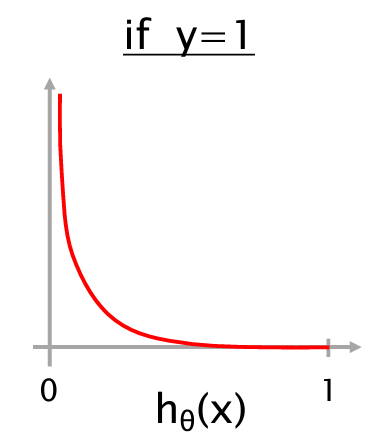
\includegraphics[scale=0.7]{img/Loss_y1.png}
    \end{center}
    \newcolumn
    \begin{center}
        \centering
        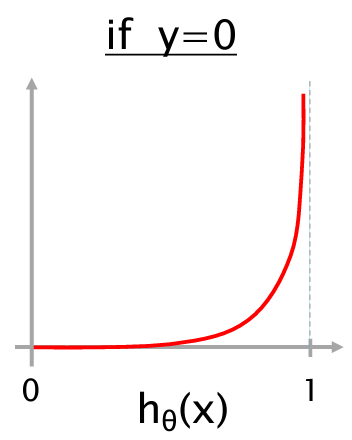
\includegraphics[scale=0.7]{img/Loss_y0.png}
    \end{center}
\end{multicols}

\noindent
Since the Loss function must penalize the objective to be effective in case the effective output is $y=1$ and the hypotesis (formulated with those parameters) would give 0, then the cost is very high. On the contrary a positive hypotesis with an actual output of $y=0$ will give to the functional a very high contribution, resulting in an high penalization (keep in mind that the functional must be minimized). This concept has a quite intuitive explanation as we have seen. \\
It would be useful having an \textit{overall functional} and with the aim of obtaining it, we badly exploit the fact that the output is logistic. In particular: 
\begin{equation}
    \text{Loss}(h(\theta),y)=-{\color{red}y} \log{h_\theta{(x)} - {\color{red}(1-y)}\log{(1-h_\theta(x))}}
\end{equation}

\noindent
The cost function coming from such a loss function is the following and it is denoted as \textbf{Binary cross-entropy cost function}:
\begin{equation} \label{eq:cross-entropy}
    J(\theta)=
    \underbrace{-\frac{1}{m}\sum_{i=1}^m \bigg[
        -{\color{black}y^{(i)}} \log{h_\theta{(x^{(i)})} - {\color{black}(1-y^{(i)})}\log{(1-h_\theta(x^{(i)}))}}
    \bigg]}_{\textsf{\color{orange}BINARY CROSS-ENTROPY COST FUNCTION}}
\end{equation}

\section{Training logistic regression}
Given the cost function (\ref{eq:cross-entropy}), we minimize it by using gradient descent algorithm, given an unknown $x$ the output is provided by using the hypotesis 
\begin{equation}
    h_\theta(x) = \frac{1}{1+e^{-\theta^\textsf{T}{x}}}
\end{equation}

\noindent
The algorithm of gradient descent follows the same step as in \textit{linear regression}, what is changed is the shape of the hypotesis $h_\theta(x)$.

\section{Multiclass classification}
Suppose we want to do a multiclass classification, for example for tagging mail as \textbf{SPAM, WORK, FRIENDS...} Can we use logistic regression in order to carry out such a task? The answer is YES, but with some modifications. In the sense that we can reformulate the problem in \textit{one class against the others}. The steps are the following: (A) We train a logistic regression classifier $h_\theta^{(i)}(x)$ in order to predict $P(y=i|x;\ \theta)$ for each class $i$. On a new input the prediction is done as follows:
\begin{equation}
    i=\arg\max_{i} h_\theta^{(i)}(x)
\end{equation}
where $i$ is the $i$-th class. Is this a good idea for a multiclass classification? Not so much! In the sense that the computational load grows of a factor $n$, with $n$ the number of classes. 

\section{Overfitting and Regularization}
In building a predictive model, there are usually two problems which we want to avoid: \textbf{underfitting and overfitting}. In the former case, provided that there are a small number of features, the learned hypotesis will not fit properly the training set. We can also say that there is an \textbf{high bias} in the data. In the latter case (overfitting) the learnt model has got excellent performances on the training set, in the limit case $J(\theta)=0$, but \textit{fails to generalize new examples}, in this case there are \textit{too many features}, so there is an \textit{high variance} in the data. \\
The configuration which is in the middle is the so-called \textit{just right}, and it is the one we want to reach aiming to have a good model. 

\begin{figure}[h]
    \centering
    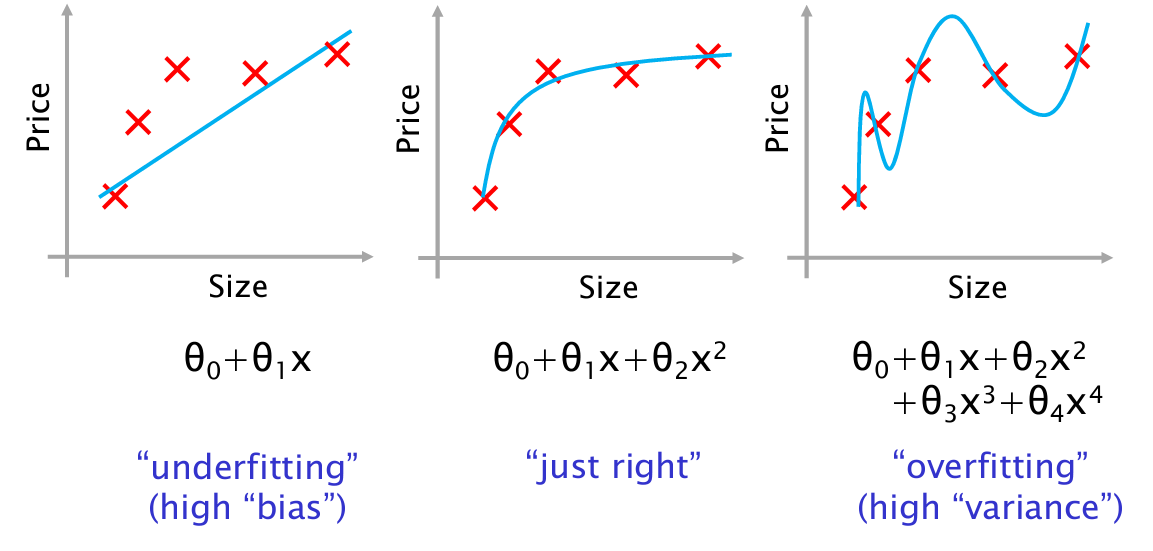
\includegraphics[scale=0.5]{img/over_under.png}
\end{figure}

\noindent
\textbf{What are the solutions for avoiding overfitting?} The first way is to reduce theb number of features the algorithm use for building the model (some techniques as PCA\footnote{
    PCA $\to$ Principal Component Analysis
} and LDA\footnote{
LDA$\to$ Linear Discriminant Analysis} can be used). Another way is introducing in the cost function a \textbf{regularization term}, its main purpose is to reduce the magnitude of the $\theta_i$ while keeping all the features. The regularization term acts directly on the parameters and it is proportional to the number of features. Using the regularization, simpler models can be obtained reducing the problem of overfitting the data. Let us consider for example the \textit{Square-error cost function}, when regularization is used it becomes:
\begin{equation} \label{eq:square_reg}
    J(\theta) = \frac{1}{2m} \sum_{i=1}^{m} (h_\theta(x^{(i)})-y^{(i)})^2 + \frac{\lambda}{2m} 
    \sum_{j=1}^{n} \theta_{j}^{2} 
\end{equation}
It is remarkable that the square-error cost function works on the $m$ training examples, while the regularization term\footnote{
    Do not confuse yourself with the \textit{normalization} which is done on the data
}interests directly the parameter of the model. The parameter $\lambda$ becomes another hyperparameter and we refer to it as the \textit{regularization parameter}. Clearly the optimization algorithm (Gradient Descent) must be updated accordingly. We also call the regularization in (\ref{eq:square_reg}) the $\ell_2$-regularization since it involves the $\ell_2$-norm definition. In the field of optimization models also the $\ell_1$-norm is considered, but in this case alternative techniques must be employed since the $\ell_1$-regularization makes the functional a non-differentiable one. Different algorithm, like ISTA and FISTA, have been developed in order to deal with such a type of optimization problem.

\chapter{Neural Networks: an introduction}
The idea of \textbf{neureal network (NN)} was introduced in the late 50s, in order to implement algorithm which could try to mimic the brain functionalities. They were very used in 80s, but their popularity decreased in the late 90s. Two determinant factors have aided the resurgence of such  technologies: the increasing in the quantity of data, and the increasing in computation capacity. For example, Neural Networks are used, among the others tasks, for performing classification.
We have understood that a linear hypotesis is not suitable for such a task, then nonlinearity is needed.\\
Now, let us imagine we want to build a model for classifying in a binary way, some images in two classes: CAR, NO CAR. An image is in general composed of pixels. Can we use \textit{logistic regression} for doing image classification? Let us consider a training set made up of $64\times{64}$ images, then 4096 pixels which is the same number for the parameter if we have a gray-scale image. If we have RGB images, the number of parameters grows by a $3$ factor, that is a number of parameters equal to $n=12288$, a huge number that makes highly unsuitable the logistic regression models. In this situation a neural network of some type is used.

\section{Ideas underlying neural networks}
Before going on through the discussion of (Artificial) Neural Networks, we have to just mention how a biological neuron is made.

\begin{figure}[h]
    \centering
    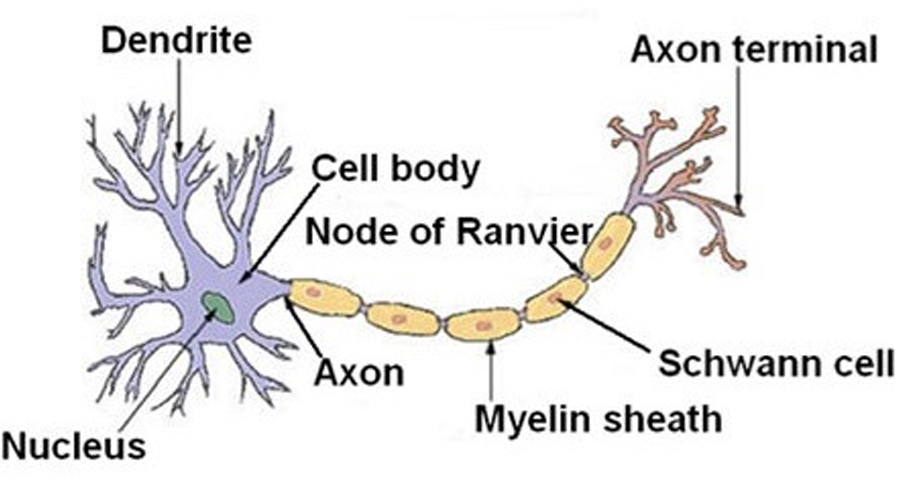
\includegraphics[scale=0.5]{img/bio_neuron.png}
\end{figure}
\noindent
Three are the main components of a neuron:
\begin{enumerate}
    \itemsep-0.2em
    \item Some inputs wires (\textbf{Dendrites})
    \item A \textbf{Nucleus} which is the \textit{computational unit}
    \item An output wire (\textbf{Axon})
\end{enumerate}
Clearly such a type of cells are connected each other by mean of \textit{synapses} realized by neutrotransmitters. \\
The \textbf{artificial neural newtork} has exactly the same structure of a biological one whose building blocks are some \textit{artificial neurons} made up of the same three basic elements, since it has got: (i) some inputs which are the features, (ii) a computation unit that performs a weighted sum of the features, (iii) an output which is the result of an \textbf{activation function} which often can be a sigmoid. [From this point we can see the strong relationship with the logistic regression.] Other activation functions can be used, besides another example is the \textbf{ReLU}.

\begin{figure}[h]
    \centering
    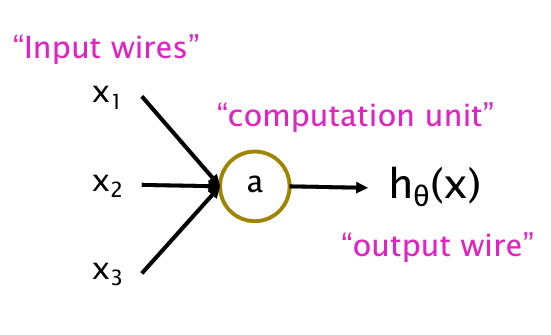
\includegraphics[scale=0.7]{img/artificialneuron.png}
    \caption{Structure of an artificial neuron}
\end{figure}

\subsection{Notation} 
In the following some notation is introduced that will be used in the remaining part of the course dealing with neural networks. When we put together some artificial neurons, what we obtained in general is a \textbf{multilayer perceptron} or \textit{classical NN}. The \textit{layer 0} is the input layer, the following are numbered as first, second layer and so on. In each layer we can find one or more computational units. For example the first layer of the showed NN has 3 computational units (without considering the unit 0 which is associated to the bias). The notation $a_i^{[j]}$ indicates the \textbf{activation} in the \textbf{i-th unit} in the \textbf{$j$-th level} of the network, while $\Theta^{[j]}$ is the weighting matrix for the  $j$-th layer of the network.\footnote{
    The intermediate layers of a neural network are called \textbf{hidden layers} since the output produced is hidden and are generated by linear and non linear combination of the features.
}
Usually also the input are renamed as \textit {zero-layer activation}, then are indicated with $a_i^{[0]}$. For the presented MLP\footnote{
    multilayer perceptron
} let us try to write all of the activation of each layer:
\begin{align*}
    &a_1^{[1]} = g(\Theta_{10}^{[1]} a_0^{[0]} + \Theta_{11}^{[1]} a_1^{[0]}+\Theta_{12}^{[1]}a_2^{[0]}+\Theta_{13}^{[1]}a_3^{[0]})=g(z_1^{[1]})\\
    &a_2^{[1]} = g(\Theta_{20}^{[1]} a_0^{[0]} + \Theta_{21}^{[1]} a_1^{[0]}+\Theta_{22}^{[1]}a_2^{[1]}+\Theta_{23}^{[1]}a_3^{[0]})=g(z_2^{[1]})\\
    &a_3^{[1]} = g(\Theta_{30}^{[1]} a_0^{[0]} + \Theta_{31}^{[1]} a_1^{[0]}+\Theta_{32}^{[1]}a_2^{[0]}+\Theta_{33}^{[1]}a_3^{[0]})=g(z_3^{[1]})\\
    &a_1^{[2]} = g(
        \Theta_{10}^{[2]}a_0^{[1]}+
        \Theta_{11}^{[2]}a_1^{[1]}+
        \Theta_{12}^{[2]}a_2^{[1]}+
        \Theta_{13}^{[2]}a_3^{[1]} 
    )=g(z_1^{[2]})
\end{align*}
\noindent
In this case the weighting matrices are for the first layer $\Theta^{[1]}\in\mathbb{R}^{3,4}$, for the second layer is $\Theta^{[2]}\in\mathbb{R}^{1,4}$.

\subsection{Different types of NN for different types of purposes}
A neural network can be used either for binary or multiclass classification. In the former case the last layer has got one neuron whose activation is 0 or 1, in the latter case we have a neuron for each class in a level that is (how we will see) the \textit{softmax layer}. Moreover a neural network is said to be \textbf{shallow} (typically) when it is made up of a number of layers which is less than seven, otherwise we have a \textbf{deep neural network}.

\begin{figure}[h]
    \centering
    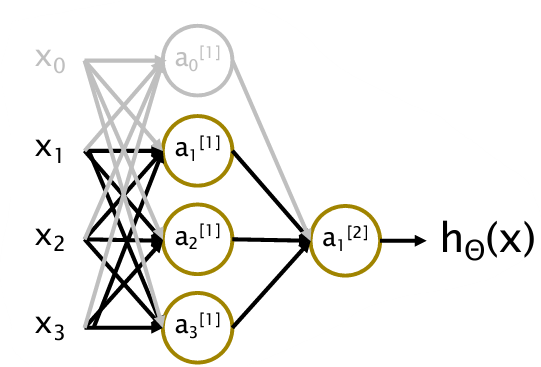
\includegraphics[scale=0.6]{img/neuron_spec.png}
\end{figure}

\section{Logistic regression as a NN}
If we better analyse the structure of a neuron and the path going from the input to the output of it, we will discover that it is something very similar to what we have seen in the case of logistic regression, where we have combined a linear part with a non linear one in order to correctly perform the (binary) classification task.\\
Now, let us suppose we want to perform a binary classification a set of images, in particular we want distinguish when they are cars or not. Can we use logistic regression in order to perform such a task? NO! It could be very slow and inefficient: a logistic regression (that is a single neuron) cannot perform in a good way such a task, then a neural network is used in this case. The next step is: how can we represent an image as a vector of features? We know that a gray-scale image can be represented as a matrix of numbers in the range [0-255], if the image is RGB we have a different matrix for each one of the channel R, G and B. We can turn the matrix into a vector by simply unrolling it row by row, in a way that each single pixel of each one of the channel is a feature for our classification problem. This example was just to present the problem of \textbf{vectorization}, that in the field of neural network is a very common operation which is done on the data in order to make them suitable for network itself.\\

\noindent
We have seen in the logistic regression that our \textbf{predicted value} $\hat{y}$ (which was the hypotesis), is nothing but the result of a sigmoidal function applied to the linear combination $w^T{x}+b$, where $w$ are the weights, $b$ is the bias while $x$ is the feature vector. Then we have that: 
\begin{equation}
    \hat{y}=a=\sigma(w^T{x}+b)
\end{equation}
How we mentioned, this is exactly the work performed by a neuron from the inputs to the output. Furthermore, we have seen that for the logistic regression a different cost function must be considered in order not to dealing with \textit{non-convex optimization problem}. For the description of the logistic regression as a single-neuron NN, nothing change a part from few differences in the notation. In fact we indicate the hypotesis $h_\theta(x)$, with the \textit{predicted value} $\hat{y}$, while the $\theta_i$ parameters are split in weights $w$ and a single bias $b$. Another difference we can find in the field of NN, is that the partial derivatives of the functional $J$ to be minimized with respect to the weights/bias, that is 
\begin{equation}
    \frac{\partial{J}}{\partial{w}}, \quad 
    \frac{\partial{J}}{\partial{b}}
\end{equation}
are denoted simply with $dw$ and $db$, in order to make lighter the notation. The \textit{gradient descent step} in order to decrease the functional becomes:
\begin{align*}
    &w = w - \alpha\ {dw}\\
    &b = b - \alpha\ {db}
\end{align*}
Now, \textbf{How can we compute the partial derivatives?} For sure, we can say that no explicit analytic calculation are performed, instead a very powerful tool that is the \textbf{automatic differentiation} leveraging on the so-called \textbf{computation graph} is used. The main concept behind it is to express a function by using \textit{intermediate auxiliary variables} and computing the derivatives by using the \textbf{Leibnitz's Chain Rule}.

\section{Automatic differentiation and computation graph}
Suppose we have a function
\begin{equation}\label{eq:exJ}
    J(a,b,c)=3(a+bc)
\end{equation}
we want to compute the ppartial derivatives of $J$ with respect to the three variables $a,b,c$. We can introduce some intermediate variables which can be called
\begin{equation*}
    u=bc \quad  v=a+u
\end{equation*}
Our function $J$ becomes: $J=3v$. In this way we have split the original function in trhee different simpler functions. This procedure can be graphically represented as shown in the figure:

\begin{figure}[h]
    \centering
    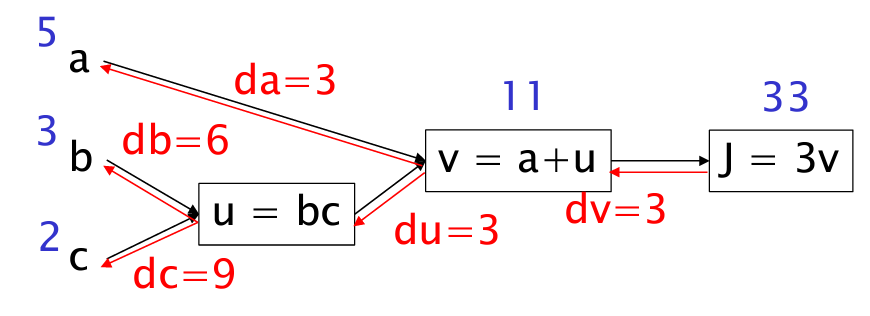
\includegraphics[scale=0.5]{img/computation_graph.png}
    \caption{Computation graph for $J=3(a+bc)$}
\end{figure}
\noindent
In particular from the input $a,b,c$, we can compute the value of the intermediate variable $u$, which can be used for obtaining $v$, finally we can compute $J$. This path from $(a,b,c)\to{J}$ is called \textbf{Forward Propagation}. Now, what about the partial derivatives? We can proceed step by step, doing an inverse path from $J\to(a,b,c)$, intuitively such a path is the \textbf{Backward propagation}, here the \textit{Chain rule} is used in order to carry out 'gradually' the computation of the partial derivatives.
The following steps are done:
\begin{align*}
    &\frac{\partial{J}}{\partial{v}}\doteq{\color{red}\mathbf{dv}}=\mathbf{\color{red}3} \quad
    \frac{\partial{J}}{\partial{u}}\doteq{\color{red}\mathbf{du}}=
    \frac{\partial{J}}{\partial{v}} \frac{\partial{v}}{\partial{u}} = 3 \cdot 1 = \mathbf{\color{red}3}\\
    &\frac{\partial{J}}{\partial{a}} \doteq{\color{red}\mathbf{da}}=
    \frac{\partial{J}}{\partial{v}} \frac{\partial{v}}{\partial{a}} = \mathbf{\color{red}3} \quad
    \frac{\partial{J}}{\partial{b}}\doteq{\color{red}\mathbf{db}}=
    \frac{\partial{J}}{\partial{v}}\frac{\partial{v}}{\partial{u}}\frac{\partial{u}}{\partial{b}}=3\cdot{1}\cdot{c}=3c=\mathbf{\color{red}6}\\
    &\frac{\partial{J}}{\partial{c}}\doteq{\color{red}\mathbf{dc}}=
    \frac{\partial{J}}{\partial{v}}\frac{\partial{v}}{\partial{u}}\frac{\partial{u}}{\partial{c}}=3\cdot{b}=\mathbf{\color{red}9}
\end{align*}
The procedure we have just shown is THE way in which are computed the derivatives in the field of Neural Network. Clearly, the same reasoning we have done for the functional (\ref{eq:exJ}) can be repeated for the \textit{loss function} used for the case of logistic regression. The figure below shows the final result of forward and backward propagation applied for the \textbf{cross-entropy loss function}.
\begin{figure}[h]
    \centering
    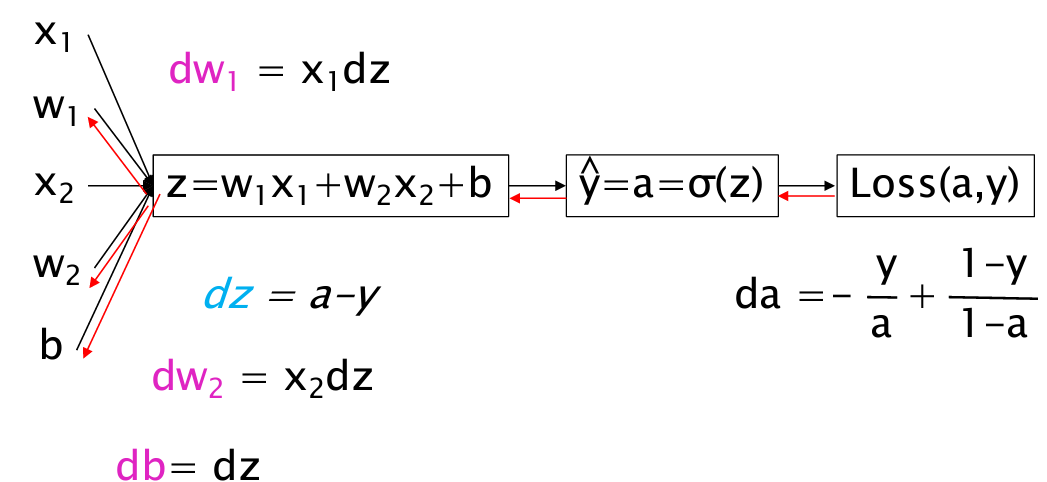
\includegraphics[scale=0.5]{img/compgraph_Loss.png}   
\end{figure}

\subsection{Feedback and Backward propagation for Logistic Regression}
For a single training sample we have that the feedback and backward propagation mathematical steps are the following:
\begin{multicols}{2}
    \noindent
    \textbf{FORWARD PROPAGATION}
    \begin{align*}
        &z_i=w^T{x^{(i)}}+b \quad \text{(linear part)}\\
        &\hat{y}_i=a_i=\sigma(z_{i})   \quad \text{(activation)}\\
        &J_{i}=-[y_{i}\log{a_{i}}+(1-y_{i})\log(1-a_{i})] \\
        & \quad \quad \text{(cost function)}
    \end{align*}
    \newcolumn\\
    \noindent
    \textbf{BACKWARD PROPAGATION}
    %\begin{align*}
        %&z=w^T{X}+b \quad \text{(linear part)}\\
        %&\hat{y}=a=\sigma(z)   \quad \text{(activation)}\\
        %&J=-\frac{1}{m}[y\log{a}+(1-y)\log(1-a)] \\
        %& \quad \quad \text{(cost function)}
    %\end{align*}
    \begin{align*}
        &dz_i = a_i-y_i\\
        &dw_i={x^{(i)}}{dz_i}\\
        &db_i=dz_i
    \end{align*}
\end{multicols}
\noindent
Whether we extend such computations to the whole dataset, we have matrices and vectors instead of vectors and scalars. In particular:
\begin{multicols}{2}
    \noindent
    \textbf{FORWARD PROPAGATION}
    \begin{align*}
        &z=w^T{X}+b \quad \text{(linear part)}\\
        &\hat{y}=a=\sigma(z)   \quad \text{(activation)}\\
        &J_{i}=-1/m \sum [y\log{a}+(1-y)\log(1-a)] \\
        & \quad \quad \text{(cost function)}
    \end{align*}
    \newcolumn\\
    \noindent
    \textbf{BACKWARD PROPAGATION}
    %\begin{align*}
        %&z=w^T{X}+b \quad \text{(linear part)}\\
        %&\hat{y}=a=\sigma(z)   \quad \text{(activation)}\\
        %&J=-\frac{1}{m}[y\log{a}+(1-y)\log(1-a)] \\
        %& \quad \quad \text{(cost function)}
    %\end{align*}
    \begin{align*}
        &dz = a-y\\
        &dw= \frac{1}{m} (X^T{dz^T})\mathbf{1}\\
        &db=\frac{1}{m}(\mathbf{1}^T{dz})
    \end{align*}
\end{multicols}
\noindent
Where $\mathbf{1}$ is a column vector with all ones. After having performed the forward and backward steps, both weights and bias must be updated as follows: 
\begin{equation}
    w:=w-\alpha\cdot{dw} \quad b:= b-\alpha\cdot{db}
\end{equation}
Such steps must be repeated until convergence (in some sense). Keep always in mind that $dw$ and $db$ are the partial derivatives of the cost function with respect to the weights and bias.

\section{Training Neural Networks}
Till now we have seen the optimization procedure of the \textit{logistic regression} as a single neuron. However, we know that a neural network is made up of several layers which in turn are composed of several neurons (computational units). The objective here is to understand how we can generalize the \textbf{optimization procedure} in the case when the whole neural network must be trained (in particular the parameters for each neuron, for each layer must be computed).

\begin{figure}[h]
    \centering
    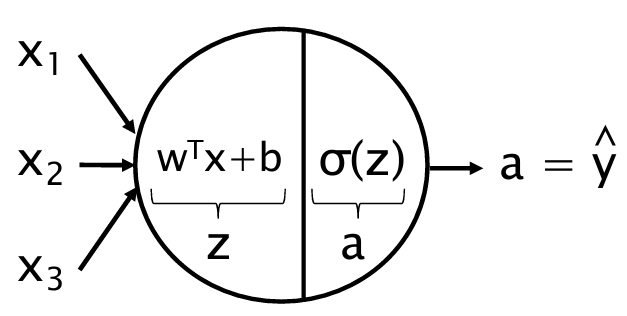
\includegraphics[scale=0.4]{img/single_log_neuron.png}
    \caption{Single neuron in form of logistic regression}
\end{figure}
\noindent
We are going to proceed step by step starting from a single neuron, going to the whole layer analyzing both the forward and backward propagations aimed to generalize the gradient descent algorithm to the whole network. For sake of simplicity but without loss of generality, the analysis has been conducted on a 2-layer NN. In the following the activation function will be indicated with $g$  in order to generalize to the use of different functions which can be used.

\subsection{Forward propagation}

\subsubsection{Single neuron, single sample}
\begin{multicols}{2}
    \begin{center}
        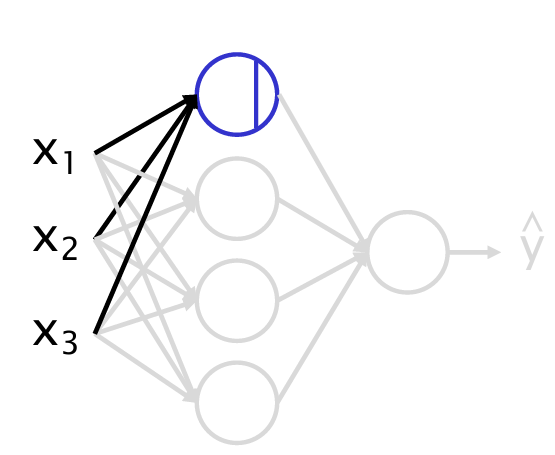
\includegraphics[scale=0.5]{img/2L_single.png}
    \end{center}
    \newcolumn
    A single neuron of the layer is considered, which clearly has his own weights and bias.
    \begin{equation} \label{eq:single_neuron}
        \begin{aligned}
            &z_1^{[1]}=w_1^{[1]T}{x}+b_1^{[1]}\\
            &a_1^{[1]}=g(z_1^{[1]})
        \end{aligned}
    \end{equation}
    The function $g$ can be something different with respect to a sigmoid. Only one sample $x$ of the dataset is considered.
\end{multicols}

\subsubsection{Single Layer, single sample}
\begin{multicols}{2}
    \begin{center}
        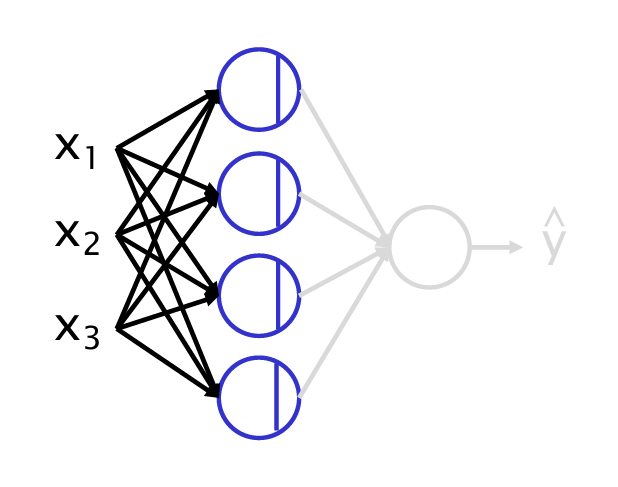
\includegraphics[scale=0.45]{img/2L_layer.png}
        \vspace{-0.5cm}
    \end{center}
    Considering all the neurons in the first layer, we have the (\ref{eq:single_neuron}) repeated four times, that is: 
    \begin{equation*}
        \begin{aligned}
            &z_i^{[1]}=w_i^{[1]T}{a^{[0]}}+b_i^{[1]}\\
            &a_i^{[1]}=g(z_i^{[1]})
        \end{aligned}, \quad i=1,...,4
    \end{equation*}
    Here the only difference is that we have indicated in terms of activations the input. In a more compact form we can say that:
    \begin{equation}
        \begin{aligned}
            &z^{[l]}=W^{[l]}a^{[l-1]}+b^{[l]}\\
            &a^{[l]}=g(z^{[l]})
        \end{aligned}
    \end{equation}
    where $l$ indicates the $l$-th layer of the network.
 \end{multicols}

\subsubsection{Single layer, whole dataset}
Till now we have seen the \textit{forward step} for a single neuron and for a layer of the network. What if considering the whole dataset instead of a single sample? The vector $z$ of the linear combination becomes a matrix in which the \textbf{$i$-th row} contains the linear combination for the \textbf{$j$-th} sample of the activation of the past layer. We have:
\begin{equation}
    \begin{aligned}
        &Z^{[l]}=W^{[l]}A^{[l-1]}+b^{[l]}\\
        &A^{[l]}=g^{[l]}(Z^{[l]})
    \end{aligned}
\end{equation}
Here is noticeable that the activation function can be different for each level of the network. This is the reason why we put the $l$ superposed also on the $g$.
\subsection{Backward propagation}
For the case of backward propagation we give directly the result in the most general case in which the loss function is even different than the \textit{cross-entropy}. Then, we have:
\begin{equation}
    \begin{aligned}
        &dZ^{[l]}=dA^{[l]}.*g^{[l]'} \ Z^{[l]}\\
        &dW^{[l]}=\frac{1}{m} (dZ^{[l]}A^{[l-1]T})\\
        &db^{[l]}=\frac{1}{m} \text{sum}({dZ^{[l]}})=\frac{1}{m}dZ^{[l]}\mathbf{1}\\
        &dA^{[l-1]}=W^{[l]T} dZ^{[l]}
    \end{aligned}
\end{equation}
For the output layer $dA^{[L]}=A^{[L]}$. The gradient step must be performed for each layer once all the derivatives have been computed: 
{\large{
    \begin{equation}
        W^{[l]}:= W^{[l]}-\alpha\cdot{dW^{[l]}} \quad    b^{[l]}:=b^{[l]}-\alpha\cdot{db^{[l-1]}}
    \end{equation} 
}}
The whole procedure of forward and backward propagation can be schematically represented by using a block diagram: 

\begin{figure}[h]
    \centering
    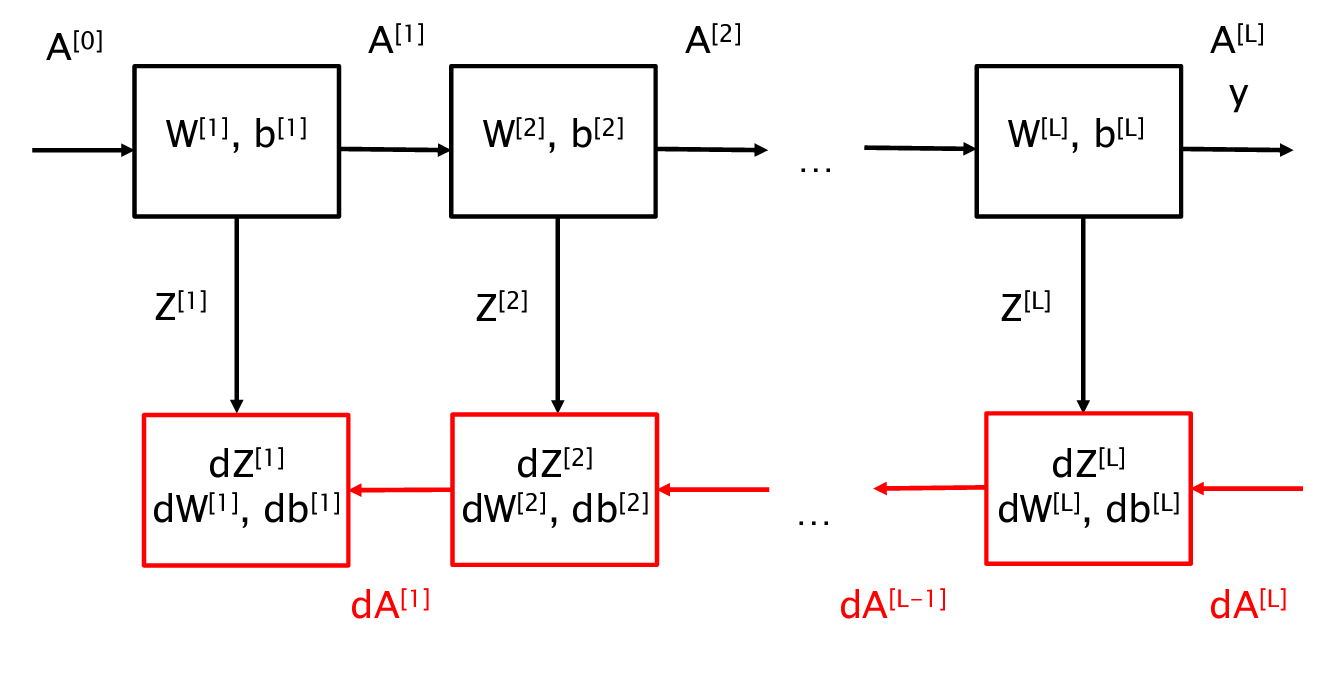
\includegraphics[scale=0.5]{img/block_diagram_GD.png}
    \caption{Block diagram for the GD}
\end{figure}

\section{Activation functions}
At different layers of a neural network, different activation functions can be used. Till now we have seen the sigmoid, since it is the one arising in the case of \textit{logistic regression}. Other choices can be done according to the needed convergence property and the task to be performed. The most common used activation functions are reported in the figure below (in the description there is also the definition).

\begin{figure}[h]
    \centering
    \subfigure[$\sigma(z)={1}/{(1+e^{-z}})$]{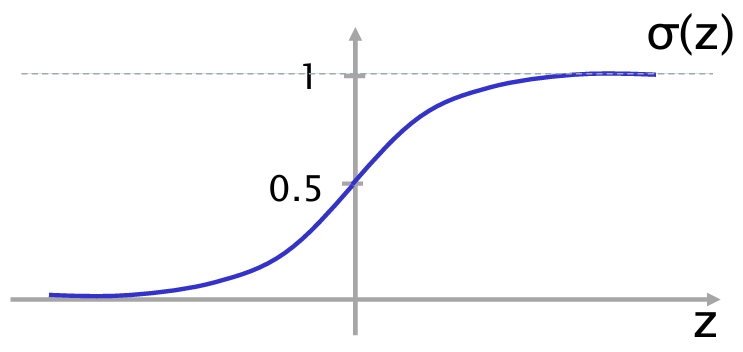
\includegraphics[scale=0.45]{img/sigmoid.png}}
    \subfigure[$\tanh(z)=(e^z-e^{-z})/(e^{z}+e^{-z})$]{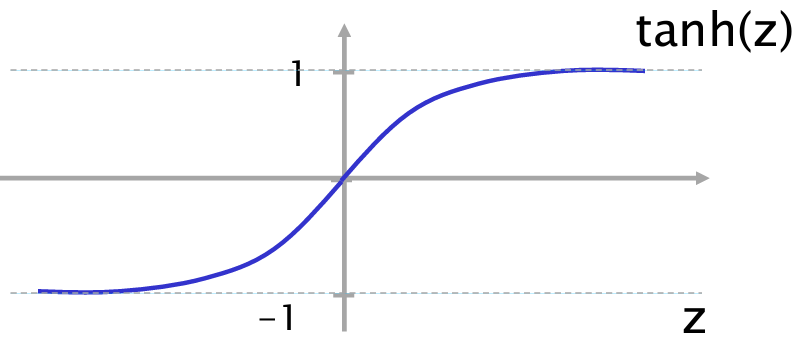
\includegraphics[scale=0.45]{img/tanh.png}}
    \subfigure[$\text{ReLU}(z)=\max(0,z)$]{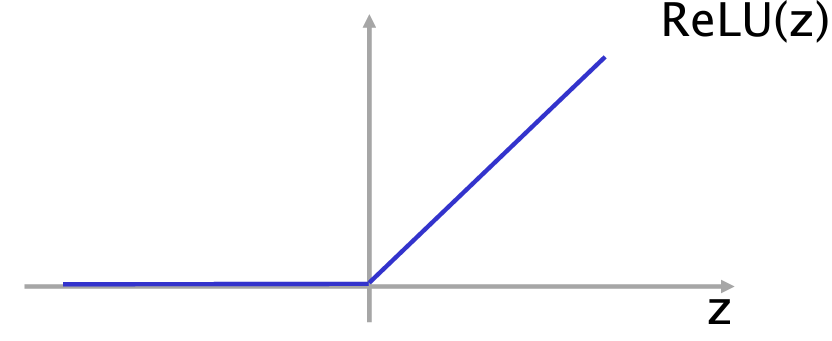
\includegraphics[scale=0.45]{img/ReLU.png}}
    \subfigure[$LeakyReLU(z)=max(\varphi{z}, z)$]{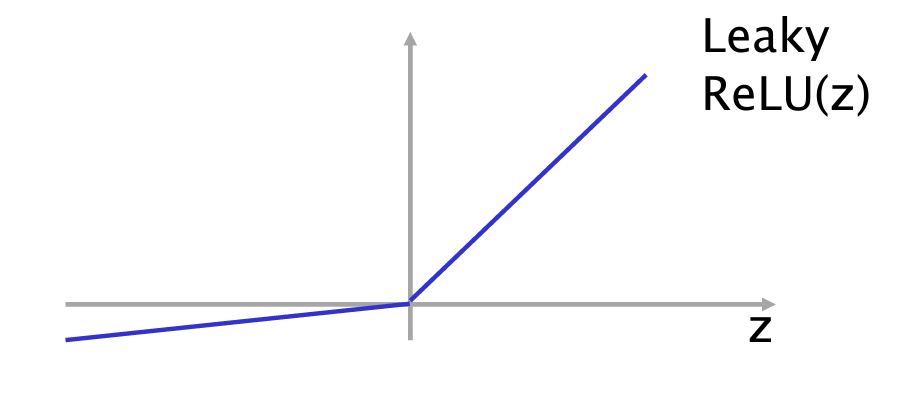
\includegraphics[scale=0.45]{img/LeakyReLU.png}}
    \caption{Some activation functions}
\end{figure}
\noindent
Note that in the $LeakyReLU(z)$ there is a parameter $\varphi$, this is in order to deal with the fact that the derivatives of $ReLU(z)$ for $z<0$ is equal to zero. Such an $\varepsilon$ becomes an hyperparameter.

\section{Initialization of the parameters}
When we have seen the \textit{linear regression} and the \textit{logistic regression}, we have said that the parameters $\theta_i$ would have been initialized for example to zero. This does not work in the case of neural networks. It has been demonstrate that the \textbf{zero-Initialization} of the weights leads to a problem of \textbf{Symmetric weights}, that is after each update, parameters associated to the inputs going to the next hidden layer unit are \textit{identical}. One possible solution, at least for simple NN, is to iniatialize randomly the weights $W^{[l]}$ and biases $b^{[l]}$ with numbers in the interval $[-\epsilon, \epsilon]$. Indeed, more sophisticated approaches are needed in the case of deep neural networks.

\section{Training a neural network (Recipe)}
Once we have presented the main issues related to neural networks and their training, we are ready to give a list of steps aimed to the training: 
\begin{enumerate}
    \itemsep-0.3em
    \item[0.] Pick a network structure, fix the numer of input and output unit with respect to number of inputs and number of classes respectively; the \textit{number of hidden layers} can be decided at this stage and also the number of neurons for each one of such layers. This are all \textbf{hyperparameters}.
    \item Randomly initialize the weights
    \item Implement \textit{forward propagation} in order to get the estimate $\hat{y}^{(i)}$ for any $x^{(i)}$;
    \item Implement code to compute the cost function $J(w,b)$ (this is another choice that we have done according to the task to be performed); 
    \item Implement \textbf{backward propagation} to compute partial derivatives (of the functional wrt the parameters);
    \item Use \textbf{gradient descent} or other optimization methods together with backward propagation to try to minimize $J(w,b)$.
\end{enumerate}

\section{Hyperparameters}
In the field of neural networks is fundamental the distinction between \textbf{parameters} and \textbf{hyperparameters}. The former ones are the ouput of the training phase, they are those that characterize a model from another. The latter ones are related to the choices that the \textit{machine learning engineer} makes in order to improve the performances of the predictive model. Examples of hyperparameters are:
\begin{itemize}
    \itemsep-0.3em
    \item Learning rate $\alpha$ of the gradient descent; 
    \item Number of iterations of the optimization algorithm; 
    \item Number of hidden layers and for each one the number of computational units; 
    \item Activation functions for each layer and related hyperparameters (eg. in the Leaky ReLU there is $\varphi$ to choose)
 \end{itemize}
 The \textbf{optimal (in some sense) configuration} must be found. 

\section{Training, Development, Test sets}
When we want to build a machine learning model, we must have a \textbf{dataset}. Clearly, since the optimal configuration of the network has to be found, only a portion of this data is used for the training phase. In general the dataset is divided into three portions:
\begin{figure}[h]
    \centering
    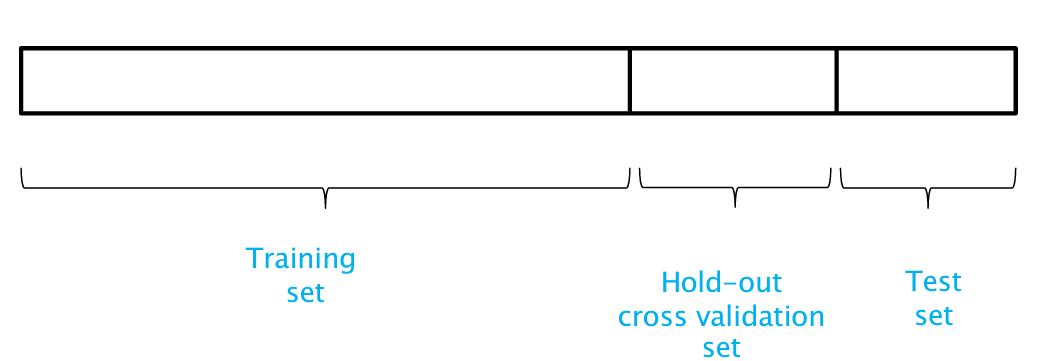
\includegraphics[scale=0.5]{img/dataset.png}
    \caption{Traditional dataset partitioning}
\end{figure}

In the past, when not too much data was available the ratios were 60\%, 20\%, 20\%; however with the increasing of the data availability the trend is using as much data as possible for the training set (98\%) and the remaining part for development and test (1\% for each one).
 \begin{description}
    \item[Training set] Is the biggest part of the dataset which is used for building the model (obtaining parameters). On this set could be necessary preliminary operations of \textit{data preparation} (eg. normalization, data augmentation and so on).
    \item[Cross-Validation/Development set] Is the set used for evaluating different models (not necessarily different architectures, but also different hyperparameters). The data distribution should match with the one in the training set. The validation set which is used, clearly is the same for all the selected models.
    \item[Test set] Once the model has been chosen a test on data that the network has never seen should be done. Such data can be extracted from the dataset, or coming from other sources making optional the presence of this type of set.
\end{description}

Once having defined how it is split the dataset, the \textbf{model selection} takes place, performing the following procedure. Given different models:
\begin{itemize}
    \item I minimize the cost function on the training set finding the parameters for each of them; 
    \item Compute the cross-validation error (on the validation set) using the output parameters for that model; 
    \item Chosse the model with the lowest error, then evaluate the \textbf{generalization performances} (using the \textit{test set}).
\end{itemize}

\chapter{Evaluating learning algorithm}

\section{Underfitting and overfitting data}
Once the model has been built, we are interested in detecting wheter out model is affected by either \textit{high bias} or \textit{high variance}. In order to better formalize such a concept is interesting to analyze the graph below: 

\begin{figure}[h]
    \centering
    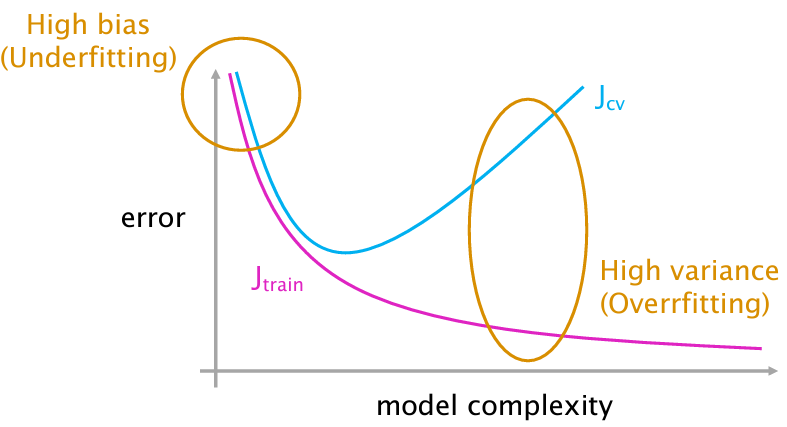
\includegraphics[scale=0.6]{img/bias_variance.png}
    \caption{High-bias vs High-variance}
\end{figure}

\noindent
Only for diagnostic purposes, we collect the data related to the error that the model does on the training data. Clearly the cost function $J_{\text{train}}$ is very high with a  very simple model because the network has not seen a sufficient amount of data. The error on the training set becomes smaller and smaller with the increasing complexity (number of features and so number of parameters of the model). What is very interesting to observe is what happen to the cost function when the validation data are used and the model complexity is growing. At start with a very simple model we have similar cost function, in fact $J_{\text{cv}}$ is very similar to $J_\text{train}$. This situation arises when the model is too simple and the model is \textbf{underfitting the data}. At the opposite when the model complexity grows there is a big difference between the two cost functions. This is related to the fact that the model has very bad performances with never seen data. In this situation we are in front of a problem of \textbf{overfitting the data}: the model has learnt by heart the data, but it is not able to generalize. \\
Both situations must be avoided, as they make a model unusable! The same reasoning can be done by a \textit{different perspective}, that is analyzing what happen to the $J_*$ in function of the dataset size. I have an \textit{high-bias} if at the end of the training phase I have a big error (\textit{with respect  to the human error}). On the other hand, I have an \textit{high-variance} if the model has bad performances on new data, or differently said, the two errors are very different. Note that, both high-variance and bias can be present in some situation. In particular in all cases when the error on training data is high and this is at the same time distant from the cross-validation error.

\begin{figure}[h]
    \centering 
    \subfigure[High-bias]{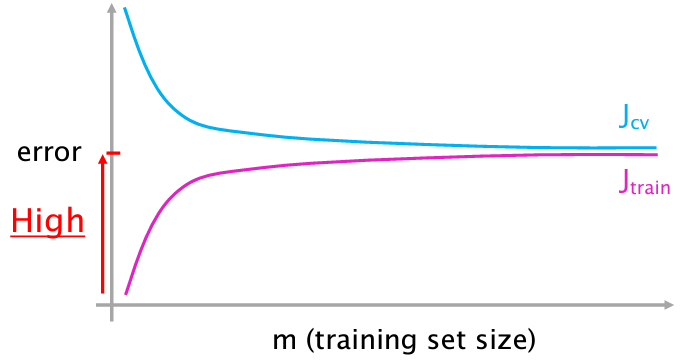
\includegraphics[scale=0.5]{img/bias_variance2.png}}
    \subfigure[High-variance]{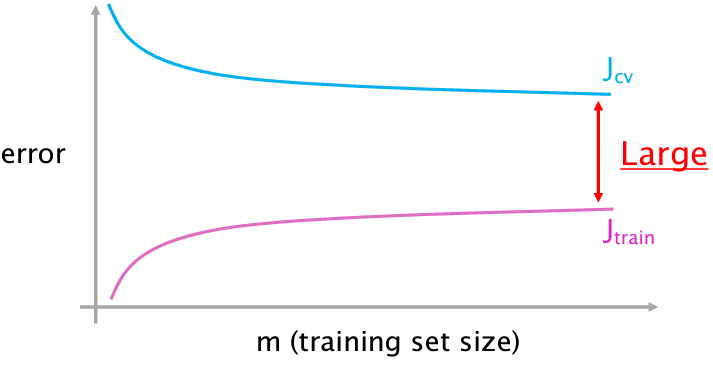
\includegraphics[scale=0.5]{img/bias_variance3.png}} 
\end{figure}

\section{Metrics for model evaluation}
\subsubsection{Motivation}
Given a model which makes a \textit{cancer classification}, suppose we want to evaluate its performance by using the so-called \textbf{accuracy}, we get a 1\% error on the validation/test set. From the labeled data, furthermore, can be analyzed for example that among all the patients only the 0.5\% has cancer. In this case if we take a \textit{Naive classifier} that ignoring the output predicts always $y=0$ (no cancer), such a classifier has better performances than the one we have properly built. The accuracy is not a good metric for evaluating the performance of a machine learning model. In this case the problem appear very evident since the data distribution is \textbf{skewed}. Conclusion: the introduction of other metrics is needed. 

\subsection{Confusion matrix and Precision/Recall}
Especially for classification tasks is useful building a matrix which compare \textit{actual and predicted} values, defining the true/false positive/negative. The one reported below is the so-called \textbf{confusion matrix}:

\begin{figure}[h]
    \centering
    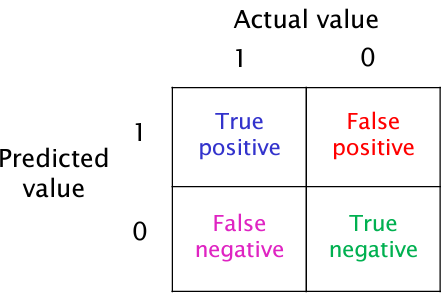
\includegraphics[scale=0.7]{img/confusion.png}
\end{figure}
\noindent
Based on the data collected in such a matrix, we can compute two different metrics: \textbf{precision} and \textbf{recall}. The former answers to the question: "Of all patient we predicted $y=1$, what portion has actually cancer?", the latter "Of all patients where we predicted $y=1$, what portion we did we correctly estimate?". In formulas:
\begin{equation}
    \text{Precision}(p)=\frac{TP}{TP+FP}\quad
    \text{Recall}(r)=\frac{TP}{TP+FN}
\end{equation}
In order to compare such metrics, another auxiliary index is introduced, the $F$ Score which is the armonic mean between recall and precision:
\begin{equation}
    F\text{-score}=\frac{pr}{p+r}
\end{equation}
Other metrics can be used, for example the \textbf{average of the diffenent accuracy indexes} in some situation can make sense, in other different situations also \textit{handcrafted} metrics can be used. It is remarkable that whether we want use eterogeneous metrics it is adviceable to maximize/minimize a single index while having the others as constraints (eg. \textit{maximize \textsf{Accuracy} subject to \textsf{Running time}$\le$100 ns})

\section{Human-level performance}
Sometimes can be useful what is the error that a human do in a classification task in order to understand on what to put the focus (ie. High-bias or high-variance or both), moreover other statistical error-rate can be computed as the \textbf{Bayes Error} which is the \textbf{lowest possible error-rate} for a given classifier. The \textit{Bayes Error} in some situation can be higher with respect to the \textit{Human-error}, this becuse by properly training a neural network the model can have the experience of several humans. Let us give an example:

\begin{figure}[h]
    \centering
    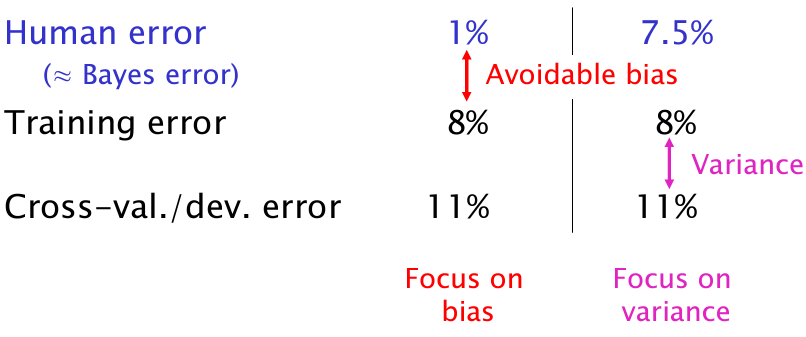
\includegraphics[scale=0.7]{img/performances.png}
\end{figure}
In the first case we can note that there is a bigger difference between the Human and Training error (here is assumed to be very similar to the Bayes error) than the one between training and validation error $\to$ we have to focus ourselves on the bias and use some strategies in order to reduce it. (This is an avoidable bias since it is mostly sufficient making the model grow to eliminate it).\\
In the second case we have similar human and training error, while there is an higher difference between the training and validation error. The most desireable thing is orthogonalize such properties which implies \textbf{having small bias while keeping low variance}, so we want them not to influencing each other (in this  sense \textit{orthogonal}).

\section{Facing bias and variance}
From a study of 2001 it appears evident that:
\begin{quotation}
    "It's not who has the best algorithm that wins, it's who has the most data" (Banko and Brill, 2001)
\end{quotation}
In principle:
\begin{itemize}
    \itemsep-0.2em
    \item In order to \textbf{reduce the bias} could be sufficient to have a \underline{\textbf{bigger model}}; 
    \item In order to \textbf{reduce the variance} could be sufficent to \underline{\textbf{use more data}} in the training phase of the model.
\end{itemize}
From a conceptual point of view it is sufficient to use the following flow-chart:

\begin{figure}[h]
    \centering
    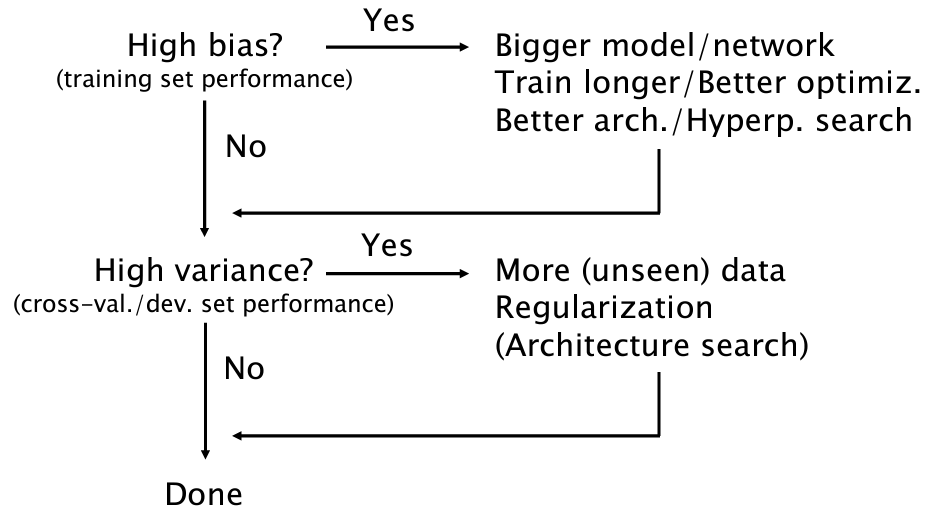
\includegraphics[scale=0.5]{img/flowchart.png}
\end{figure}
\noindent
The real-world examples demonstrates that variance and bias cannot be orthogonalized, then there is a \textbf{trade-off} to manage.


\chapter[Large Datasets and CNN]{Large Datasets and Convolutional Neural Networks (CNN)}


\end{document}